\makeatletter
\@removefromreset{figure}{section}
\@addtoreset{figure}{chapter}
\renewcommand{\thefigure}{\thechapter.\@arabic\c@figure}
\makeatother

\hypertarget{the-cloud-lab}{%
\section{The Cloud Lab}\label{the-cloud-lab}}

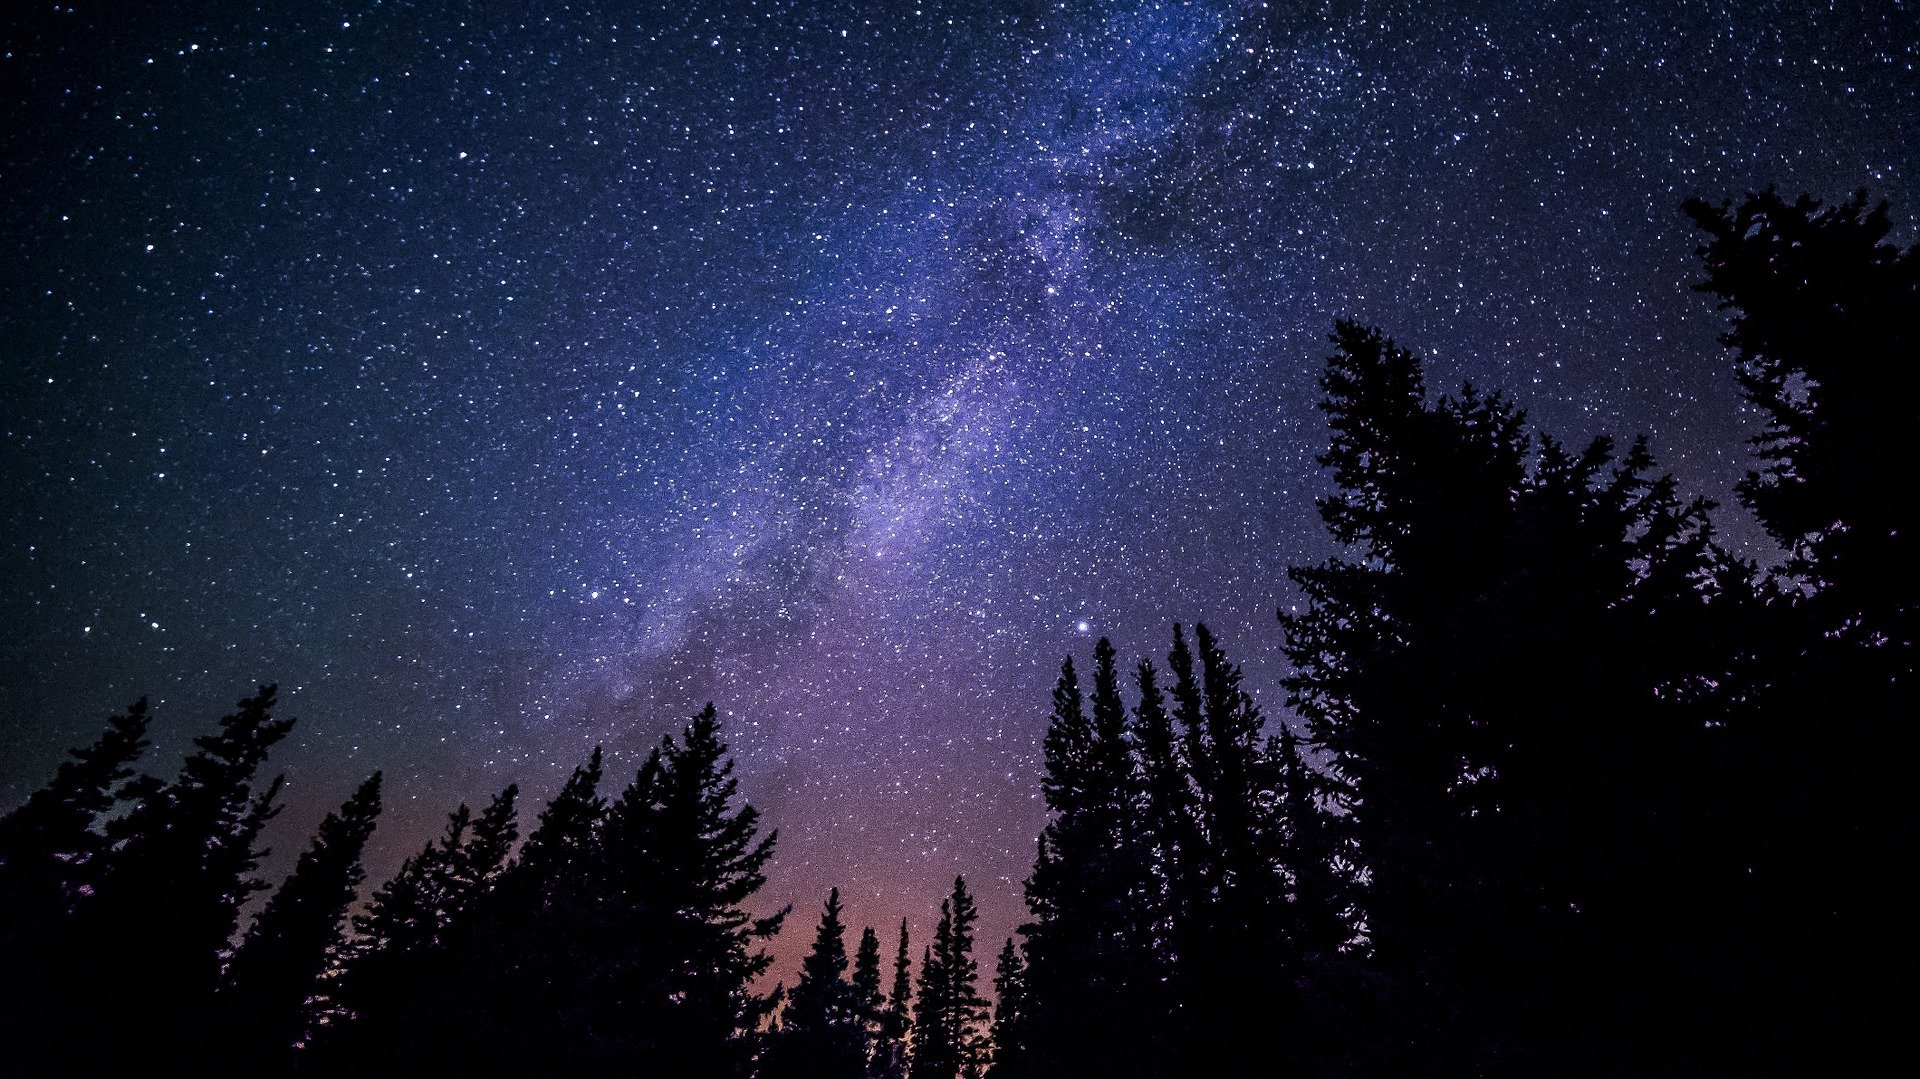
\includegraphics{../images/milky-way-984050_1920.jpg}

We've reached the point where it's time to assemble all our functional
blocks into a proper lab using resources of a cloud service provider.

\hypertarget{getting-started}{%
\subsection{Getting Started}\label{getting-started}}

\hypertarget{setting-up-aws}{%
\subsubsection{Setting up AWS}\label{setting-up-aws}}

Establish an AWS account.

\hypertarget{install-docker}{%
\subsubsection{Install Docker}\label{install-docker}}

Install Docker on your local machine. Create a Dockerfile and
docker-compose.yml.

\hypertarget{set-up-github-account}{%
\subsubsection{Set Up GitHub Account}\label{set-up-github-account}}

Create a GitHub account, Generate a SSH key and GPG key. Add to GitHub

\hypertarget{configure-project-repository}{%
\subsubsection{Configure Project
Repository}\label{configure-project-repository}}

Create a GitHub repo for our project. Clone the repo. Copy the
Dockerfile and docker-compose.yml into the new project directory. Create
a branch. Commit the files to the branch and push to repo on GitHub.
Merge the branch, then do a pull to sync your local clone.

\hypertarget{configure-testing}{%
\subsubsection{Configure Testing}\label{configure-testing}}

Walk through the steps of adding GitHub Actions that will validate the
Terraform we will be writing to establish our lab infrastructure.

\hypertarget{infrastructure}{%
\subsection{Infrastructure}\label{infrastructure}}

\hypertarget{lab-diagram}{%
\subsubsection{Lab Diagram}\label{lab-diagram}}

Let's take a look at the lab environment we intend to create.

\hypertarget{add-a-makefile}{%
\subsubsection{Add a Makefile}\label{add-a-makefile}}

Add a Makefile that will respond to the "make docker" command.

\hypertarget{create-a-host-with-packer}{%
\subsubsection{Create a Host with
Packer}\label{create-a-host-with-packer}}

\hypertarget{write-some-terraform-files}{%
\subsubsection{Write Some Terraform
Files}\label{write-some-terraform-files}}

\hypertarget{applications}{%
\subsection{Applications}\label{applications}}

\hypertarget{python-application}{%
\subsubsection{Python Application}\label{python-application}}

\hypertarget{extras}{%
\subsection{Extras}\label{extras}}

\hypertarget{add-a-firewall}{%
\subsubsection{Add a Firewall}\label{add-a-firewall}}

Every keep needs walls around the castle to stop the bad guys from
getting in. The Palo Alto VM-300 series firewall is available as an
image that can be installed in AWS or GCP as desired.
